\chapter{Clasificación con Deep Learning}\label{cap.clasificacion}
En este capítulo se expondrá el trabajo realizado para el entendimiento del problema de clasificación, mediante la elaboración de un componente en Python que permite la clasificación de dígitos del 0 al 9 en tiempo real, y la realización de un amplio estudio sobre las variantes posibles aplicadas a las redes entrenadas, utilizando la plataforma Caffe.\\
\section{Clasificador de dígitos}
Se ha desarrollado un componente en Pyhton para la clasificación de dígitos entre 0 y 9 en tiempo real, siendo necesario, previamente, un entendimiento de una primera red básica, utilizada por el mismo para la tarea. En esta sección se explicará el procedimiento seguido para el entendimiento de la red y el desarrollo del propio componente.\\
\subsection{Red básica}
La red que se empleará, está orientada a la clasificación de números utilizando, en el entrenamiento, la base de datos numérica MNIST, explicada en el Capítulo~\ref{cap.infraestructura}.\\
Para realizar el entrenamiento de la red, Caffe proporciona tres archivos que se editarán para adaptar la red al problema que se abarque. A continuación, se explicará cada uno de esos archivos, siguiendo el orden que fue necesario hasta conseguir la red completamente entrenada.
\vspace{15pt}
\begin{description}
	\item[Definición de la red] \hfill 
	\vspace{10pt}
	\\
	Caffe utiliza el archivo 
	\textit{lenet\_train\_test.prototxt} para la especificación de todos los parámetros que son necesarios en el entrenamiento de la red, es decir, define las imágenes que se emplearán, la propia estructura de la red y la forma en la que se analizarán las imágenes proporcionadas, todo ello empleando diferentes capas (\textit{layers}).\\
	\vspace{-10pt}
	\\
	La primera línea de este documento es utilizada para indicar el nombre que se le quiere dar a la red.
	\vspace{10pt}
	\begin{lstlisting}[frame=single]
	name: "LeNet"
	\end{lstlisting}
	
	En concreto, esta red recibe el nombre de LeNet, un tipo de red que es conocida por un buen funcionamiento en las tareas de clasificiación de dígitos y que, por lo general, consta de una capa convolucional seguida por una capa de agrupamiento (\textit{pooling}), repetido dos veces y, finalmente, dos capas totalmente conectadas similares a las perceptrones multicapa convencionales. En el ejemplo de Caffe, la estructura habitual de la red LeNet se ve ligeramente modificada, ya que en lugar de emplear una función de activacion sigmoidal se utiliza una linear.\\
	\vspace{-10pt}
	\\
	Tras la definición del nombre se definen dos capas de datos, una de ellas correspondiente a los datos de entrenamiento de la red y, la otra, correspondiente a los datos que se utilizarán para realizar el test durante el entrenamiento para obtener datos de \textit{accuracy} y \textit{loss}.
	\vspace{10pt}
	\begin{lstlisting}[frame=single]
	layer {
		name: "mnist"
		type: "Data"
		top: "data"
		top: "label"
		include {phase: TRAIN}
		transform_param {scale: 0.00390625}
		data_param {
			source: "examples/mnist/mnist_train_lmdb"
			batch_size: 64
			backend: LMDB
		}
	}
	\end{lstlisting}
	
	Es importante que los parámetros de transformación, en este caso un factor de escala que establece el rango de la imagen en [0,1], sean los mismos en ambas fases, pues si se evaluase la red con una transformación de la imágen distinta a la aplicada en el entrenamiento los resultados obtenidos no serían reales.\\
	Se utilizará, por tanto, dos capas de datos que difieren en la fase en la que se utilizarán los datos, entrenamiento o evaluación de la red, el tamaño del lote, siendo 64 muestras para el entrenamiento y 100 para el test, y la ruta de la que se cogen los datos.\\
	\vspace{-10pt}
	\\
	A continuación, se comienzan a definir las capas del entrenamiento propiamente dicho. Se intercala una capa de convolución con una de agrupamiento y se repite dos veces.
	\vspace{10pt}
	\begin{lstlisting}[frame=single]
	layer {
		name: "conv1"
		type: "Convolution"
		bottom: "data"
		top: "conv1"
		param {lr_mult: 1}
		param {lr_mult: 2}
		convolution_param {
			num_output: 20
			kernel_size: 5
			stride: 1
			weight_filler {type: "xavier"}
			bias_filler {type: "constant"}
		}
	}	
	\end{lstlisting}

	En la capa de convolución, explicada en el Capítulo~\ref{cap.infraestructura}, se define que el tamaño del filtro será de 5x5 y que se obtendrán 20 salidas, en la segunda capa de convolución, sin embargo, se obtendrán 50 salidas. Además se define el algoritmo "Xavier" para la inicialización de los pesos, que determina automáticamente la escala de inicialización basada en el número de entradas y de las neuronas de salida, y la inicialización del \textit{bias} mediante una constante que por defecto es 0.
	\vspace{10pt}
	\begin{lstlisting}[frame=single]
	layer {
		name: "pool1"
		type: "Pooling"
		bottom: "conv1"
		top: "pool1"
		pooling_param {
			pool: MAX
			kernel_size: 2
			stride: 2
		}
	}	
	\end{lstlisting}
	
	La capa de agrupamiento, también explicada en el Capítulo~\ref{cap.infraestructura}, será alimentada por la capa de convolución anterior y alimentará a la siguiente en caso de que la haya. Se definen en ella un tamaño de filtro de 2x2, un intervalo de dos muestras entre cada aplicación del filtro, por lo que no hay solape, y el método del máximo para realizar el agrupamiento.\\
	\vspace{-10pt}
	\\
	Tras estas capas, se establecen dos capas completamente conectadas, \textit{InnerProduct}, separadas por la capa de activación, \textit{ReLu}, ambas explicadas en el Capítulo~\ref{cap.infraestructura}. 
	\vspace{10pt}
	\begin{lstlisting}[frame=single]
	layer {
		name: "ip1"
		type: "InnerProduct"
		bottom: "pool2"
		top: "ip1"
		param {lr_mult: 1}
		param {lr_mult: 2}
		inner_product_param {
			num_output: 500
			weight_filler {type: "xavier"}
			bias_filler {type: "constant"}
		}
	}	
	\end{lstlisting}
	
	\begin{lstlisting}[frame=single]
	layer {
		name: "relu1"
		type: "ReLU"
		bottom: "ip1"
		top: "ip1"
	}	
	\end{lstlisting}
	
	Las capas completamente conectadas se definen con, 500 salidas la primera de ellas, y tantas como clases se tengan en la segunda, en el caso concreto que se trata serán 10, correspondientes con los dígitos del 0 al 9.\\
	\vspace{-10pt}
	\\
	Para terminar la estructura de la red básica, Caffe permite la opción de añadir capas que muestren parámetros de evaluación de la red que se está entrenando. Para ello, en el Capítulo~\ref{cap.infraestructura}, se explicaron varias capas de \textit{Loss}, que serán empleadas en esta red para su evaluación, se deberán explicitar en este documento.
	\vspace{10pt}
	\begin{lstlisting}[frame=single]
	layer {
		name: "accuracy"
		type: "Accuracy"
		bottom: "ip2"
		bottom: "label"
		top: "accuracy"
		include {phase: TEST}
	}
	
	layer {
		name: "loss"
		type: "SoftmaxWithLoss"
		bottom: "ip2"
		bottom: "label"
		top: "loss"
	}	
	\end{lstlisting}
	
	Estas dos capas permiten obtener valores de precisión y pérdidas cada ciertas iteraciones, siendo marcado este valor en el siguiente documento.\\
	\vspace{-10pt}
	\\
	En la Figura~\ref{fig.redBasica} se puede observar un esquema de la estructura definida en este apartado, los valores de interés y cada una de las entradas y salidas de las capas.
	
	\begin{figure}[h!]
		\begin{center}
			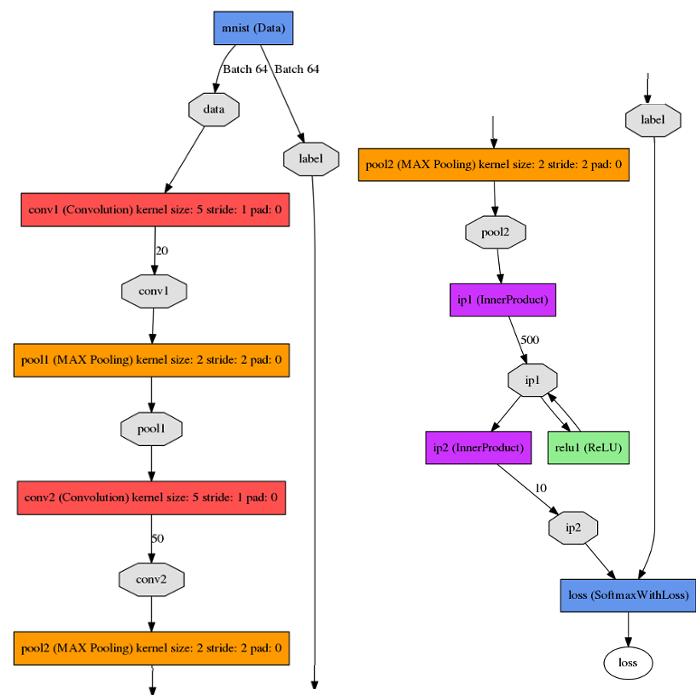
\includegraphics[width=0.8\textwidth]{figures/Original_net}
			\caption{Red básica LeNet MNIST}
			\label{fig.redBasica}
		\end{center}
	\end{figure}
	
	Para obtener la Figura~\ref{fig.redBasica}, se ha ejecutado un código proporcionado por la propia plataforma, que, mediante el archivo que define la estructura, explicado anteriormente, dibuja la red. Para ello se debe ejecutar el siguiente comando:
	\vspace{10pt}
	\begin{lstlisting}[frame=single]
	$ caffe/python/draw_net.py <netprototxt_filename> <out_img_filename>
	\end{lstlisting}
	
	\vspace{50pt}
	\item[Definición del solucionador] \hfill 
	\vspace{10pt}
	\\
	Para esta tarea se va a utilizar el archivo de Caffe \textit{lenet\_solver.prototxt}, que permitirá manejar parámetros del propio entrenamiento de la red.\\ 
	Se definen en él parámetros como la estructura de red que se utilizará, definida en el apartado anterior, y el número de iteraciones que se ejecutarán durante el entrenamiento de la red, cuya explicación se aportó en el Capítulo~\ref{cap.infraestructura}. Además, en ese mismo capítulo, se explican el resto de parámetros que se manejarán en este proyecto, como la evaluación de la red o las redes intermedias que se guardarán.
	\vspace{5pt}
	\begin{lstlisting}[frame=single]
	# The train/test net protocol buffer definition
	net: "examples/mnist/lenet_train_test.prototxt"
	# test_iter specifies how many forward passes the test should carry 
	# out.
	# In the case of MNIST, we have test batch size 100 and 100 test
	# iterations, covering the full 10,000 testing images.
	test_iter: 100
	# Carry out testing every 500 training iterations.
	test_interval: 500
	# The base learning rate, momentum and the weight decay of the network.
	base_lr: 0.01
	momentum: 0.9
	weight_decay: 0.0005
	# The learning rate policy
	lr_policy: "inv"
	gamma: 0.0001
	power: 0.75
	# Display every 100 iterations
	display: 100
	# The maximum number of iterations
	max_iter: 10000
	# snapshot intermediate results
	snapshot: 5000
	snapshot_prefix: "examples/mnist/lenet"
	# solver mode: CPU or GPU
	solver_mode: CPU	
	\end{lstlisting}
	\vspace{15pt}
	\item[Ejecución de la red] \hfill 
	\vspace{10pt}
	\\
	Una vez se han definido los parámetros adecuados para la red que se quiera entrenar, se ejecutarán los siguientes comandos, que comenzará con el entrenamiento de la red:
	\vspace{10pt}
	\begin{lstlisting}[frame=single]
	cd $CAFFE_ROOT
	./examples/mnist/train_lenet.sh	
	\end{lstlisting}
	
	El archivo que se ejecuta contiene información sobre qué solucionador se debe implementar y el modo de ejecución. Además es posible añadirle una línea que guardará un archivo con información de \textit{log} del proceso de entrenamiento.
	\vspace{10pt}
	\begin{lstlisting}[frame=single]
	#!/usr/bin/env sh
	set -e
	
	./build/tools/caffe train 
	  --solver=examples/mnist/lenet_solver_validation.prototxt 
	    2>&1 | tee /home/nuria/TFG/logs/RedBasica.log $@
	\end{lstlisting}
	
	\begin{figure}[h!]
		\begin{center}
			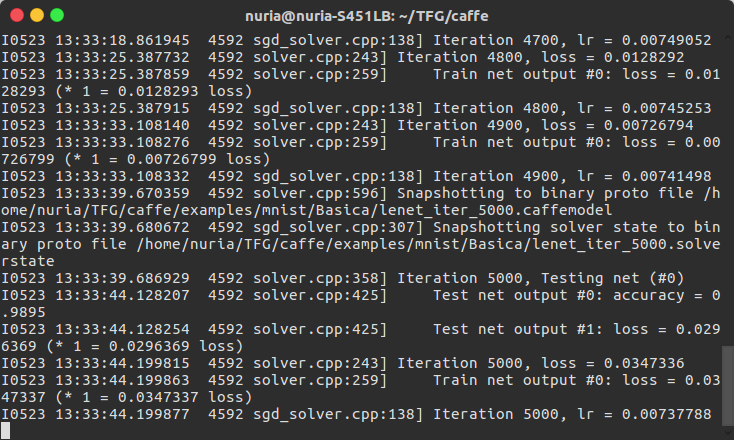
\includegraphics[width=0.8\textwidth]{figures/RedBasica5000}
			\caption{Ejecución de entrenamiento de red LeNet MNIST}
		\end{center}
	\end{figure}
	
	\begin{figure}[h!]
		\begin{center}
			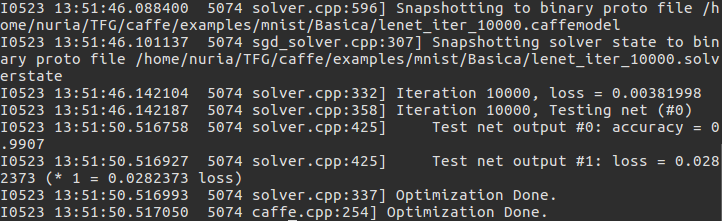
\includegraphics[width=0.8\textwidth]{figures/RedBasicaFin}
			\caption{Fin de entrenamiento de red LeNet MNIST}
			\label{fig.finEntrBas}
		\end{center}
	\end{figure}
	\vspace{30pt}
	Tras terminar el entrenamiento, mostrado en la Figura~\ref{fig.finEntrBas}, se obtiene el archivo con la red neuronal entrenada, almacenado según la ruta que se indicó en el solucionador, que podrá ser utilizada en la herramienta que sea de interés.\\
	\vspace{-10pt}
	\\
	El archivo \textit{log} generado podrá ser visualizado mediante la ejecución del script \textit{plot\_learning\_curve.py} \footnote{https://github.com/adilmoujahid/deeplearning-cats-dogs-tutorial/blob/master/code/plot\_learning\_curve.py} de la siguiente forma:
	\vspace{10pt}
	\begin{lstlisting}[frame=single]
	python plot_learning_curve.py /home/nuria/TFG/logs/RedBasica.log 
	 RedBasicaLog.png
	\end{lstlisting}
	
	En la Figura~\ref{fig.Log} se puede observar el resultado final de la curva de aprendizaje, con valores de precisión y pérdidas, según lo explicado en el Capítulo~\ref{cap.infraestructura}, para la fase de evaluación, y en entrenamiento únicamente de pérdidas.
	
	\begin{figure}[h!]
		\begin{center}
			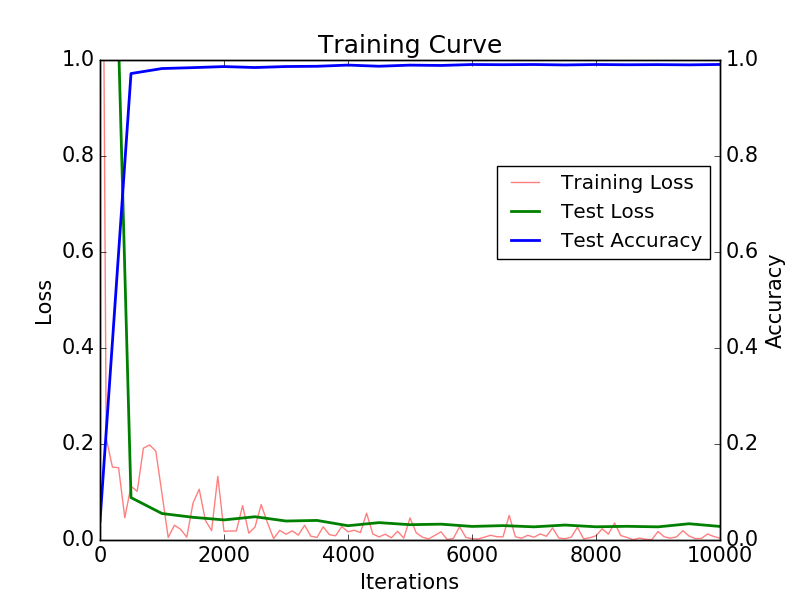
\includegraphics[width=0.5\textwidth]{figures/RedBasicaLog}
			\caption{Curva de aprendizaje Red Básica}
			\label{fig.Log}
		\end{center}
	\end{figure}
\end{description}
\subsection{Componente Python}


